\section{On-chain Protocol}\label{sec:on-chain}

We describe the details of the \emph{on-chain} protocol controlling a
Hydra head (see Fig.~\ref{fig:SM_states_basic}) using the CEM abstraction \&
notation (see Section~\ref{sec:cem}). In addition of standard CEM modeling, we
also provide the formal conditions $\cemTxCon$ which a transition need to
satisfy and also include them in the accompanying text.

The following sections describe the structure of each of the transactions
comprising the Head protocol: $\mtxInit{}$, $\mtxCom{}$, $\mtxAbort{}$,
$\mtxCollect{}$, $\mtxClose{}$, $\mtxContest{}$, and $\mtxFanout{}$. Following
the EUTxO model, this structure is enforced on-chain through \emph{validators}
which are \emph{scripts instances} attached to each UTxO and run as part of the
ledger's validation of the transaction (see Section~\ref{sec:eutxo}). The
protocol defines one minting policy script and three validator scripts:
\begin{itemize}
  \item $\muHead$ governs the minting of state and participation tokens,
  \item $\nuInitial$ controls initialization and how UTxOs are committed to the head, while
  \item $\nuCommit$ controls the collection of committed UTxOs into the head, and lastly
  \item $\nuHead$ controls the main protocol state-machine logic.
\end{itemize}

\subsection{Init transaction}

The \mtxInit{} transaction creates a head instance and establishes the initial
state of the protocol and is shown in Figure~\ref{fig:SM_commit_tx}. The head
instance is represented by the unique\footnote{As the EUTxO ledger preventing
  double-spending, the uniqueness of $\cid$ is guaranteed because $i_{seed}$ can
  only be spent once} currency identifier $\cid$ created by minting tokens using
the parameterized $\muHead$ minting policy script:
\[
  \cid = \hash(\muHead(i_{seed}))
\]
\noindent where $i_{seed} \in \txInputs$ is a transaction input and the
$\muHead(i_{seed})$ minting policy validator checks:
\begin{menumerate}
  \item $i_{seed}$ is spent in this transaction
  $i_{seed} \in \txInputs$
\end{menumerate}

\vspace{0.1cm}
\noindent Two kinds of tokens are minted:
\begin{itemize}
  \item A single \emph{State Thread (ST)} token marking the output carrying the state
        of the protocol on-chain, whose name is the well known string
        \texttt{HydraHeadV1}, i.e.
        $\st = (\cid \rightarrow \texttt{HydraHeadV1} \rightarrow 1)$\todo{$\st = (\cid \rightarrow \texttt{HydraHeadV1}$}
  \item One \emph{Participation Token (PT)} per participant
        $i \in \{1 \dots \nop \}$, where the token name is the participant's
        verification key hash $\keyHash_{i}$, i.e.
        $\pt_{i} = (\cid \rightarrow \keyHash_{i} \rightarrow 1)$.\todo{$\pt = (\cid \rightarrow \keyHash_{i})$}
\end{itemize}

\noindent Consequently, the \mtxInit{} transaction

\begin{itemize}
  \item has at least input $i_{seed}$,
  \item mints one $\st$ and one $\pt$ for each of the $\nop$ participants with
        policy $\cid :: \{\st, \pt_{1}, \ldots, \pt_{\nop}\}$,
  \item has one state-machine output locked by $\nuHead$ with datum
        $\datum_{\mathsf{head}}$
  \item has $\nop$ outputs, where each output is locked by $\nuInitial$ and the
        $\ith i$ output has the participation token $\pt_i$ in its value, and
        $\cid$ as datum.
\end{itemize}

\noindent The initial state of the protocol is captured in the state-machine output datum
\[
  \datum_{\mathsf{head}} = (\stInitial,\cid,\hpAK,\hppuv,\nop,\cPer)
\]
where
\begin{mitemize}
  \item $\stInitial$ is a state identifier,
  \item $\cid$ is the unique currency id of this instance,
  \item $\hpAK$ is the aggregated off-chain multi-signature key established during the
  setup phase,
  \item $\hppuv$ is the list of all participants verification keys
  $(k_1,\ldots,k_\nop)$ exchanged during the setup phase and identifying the
  head members on-chain,
  \item $\nop$ is the number of head participants, and
  \item $\cPer$ is the length of the contestation period.
\end{mitemize}

\noindent Validator $\nuInitial$ ensures that the output is consumed by either
an \mtxAbort{}~\ref{sec:abort-tx} or a \mtxCom{}~\ref{sec:commit-tx}
transaction. Note that the general well-formedness and validity of the
\mtxInit{} transaction is checked on the mainchain, but head members need to
additionally check whether the initial state has the right $\cid$ and is
consistent with parameters agreed during setup.

\begin{figure}[h]

  \centering

  % 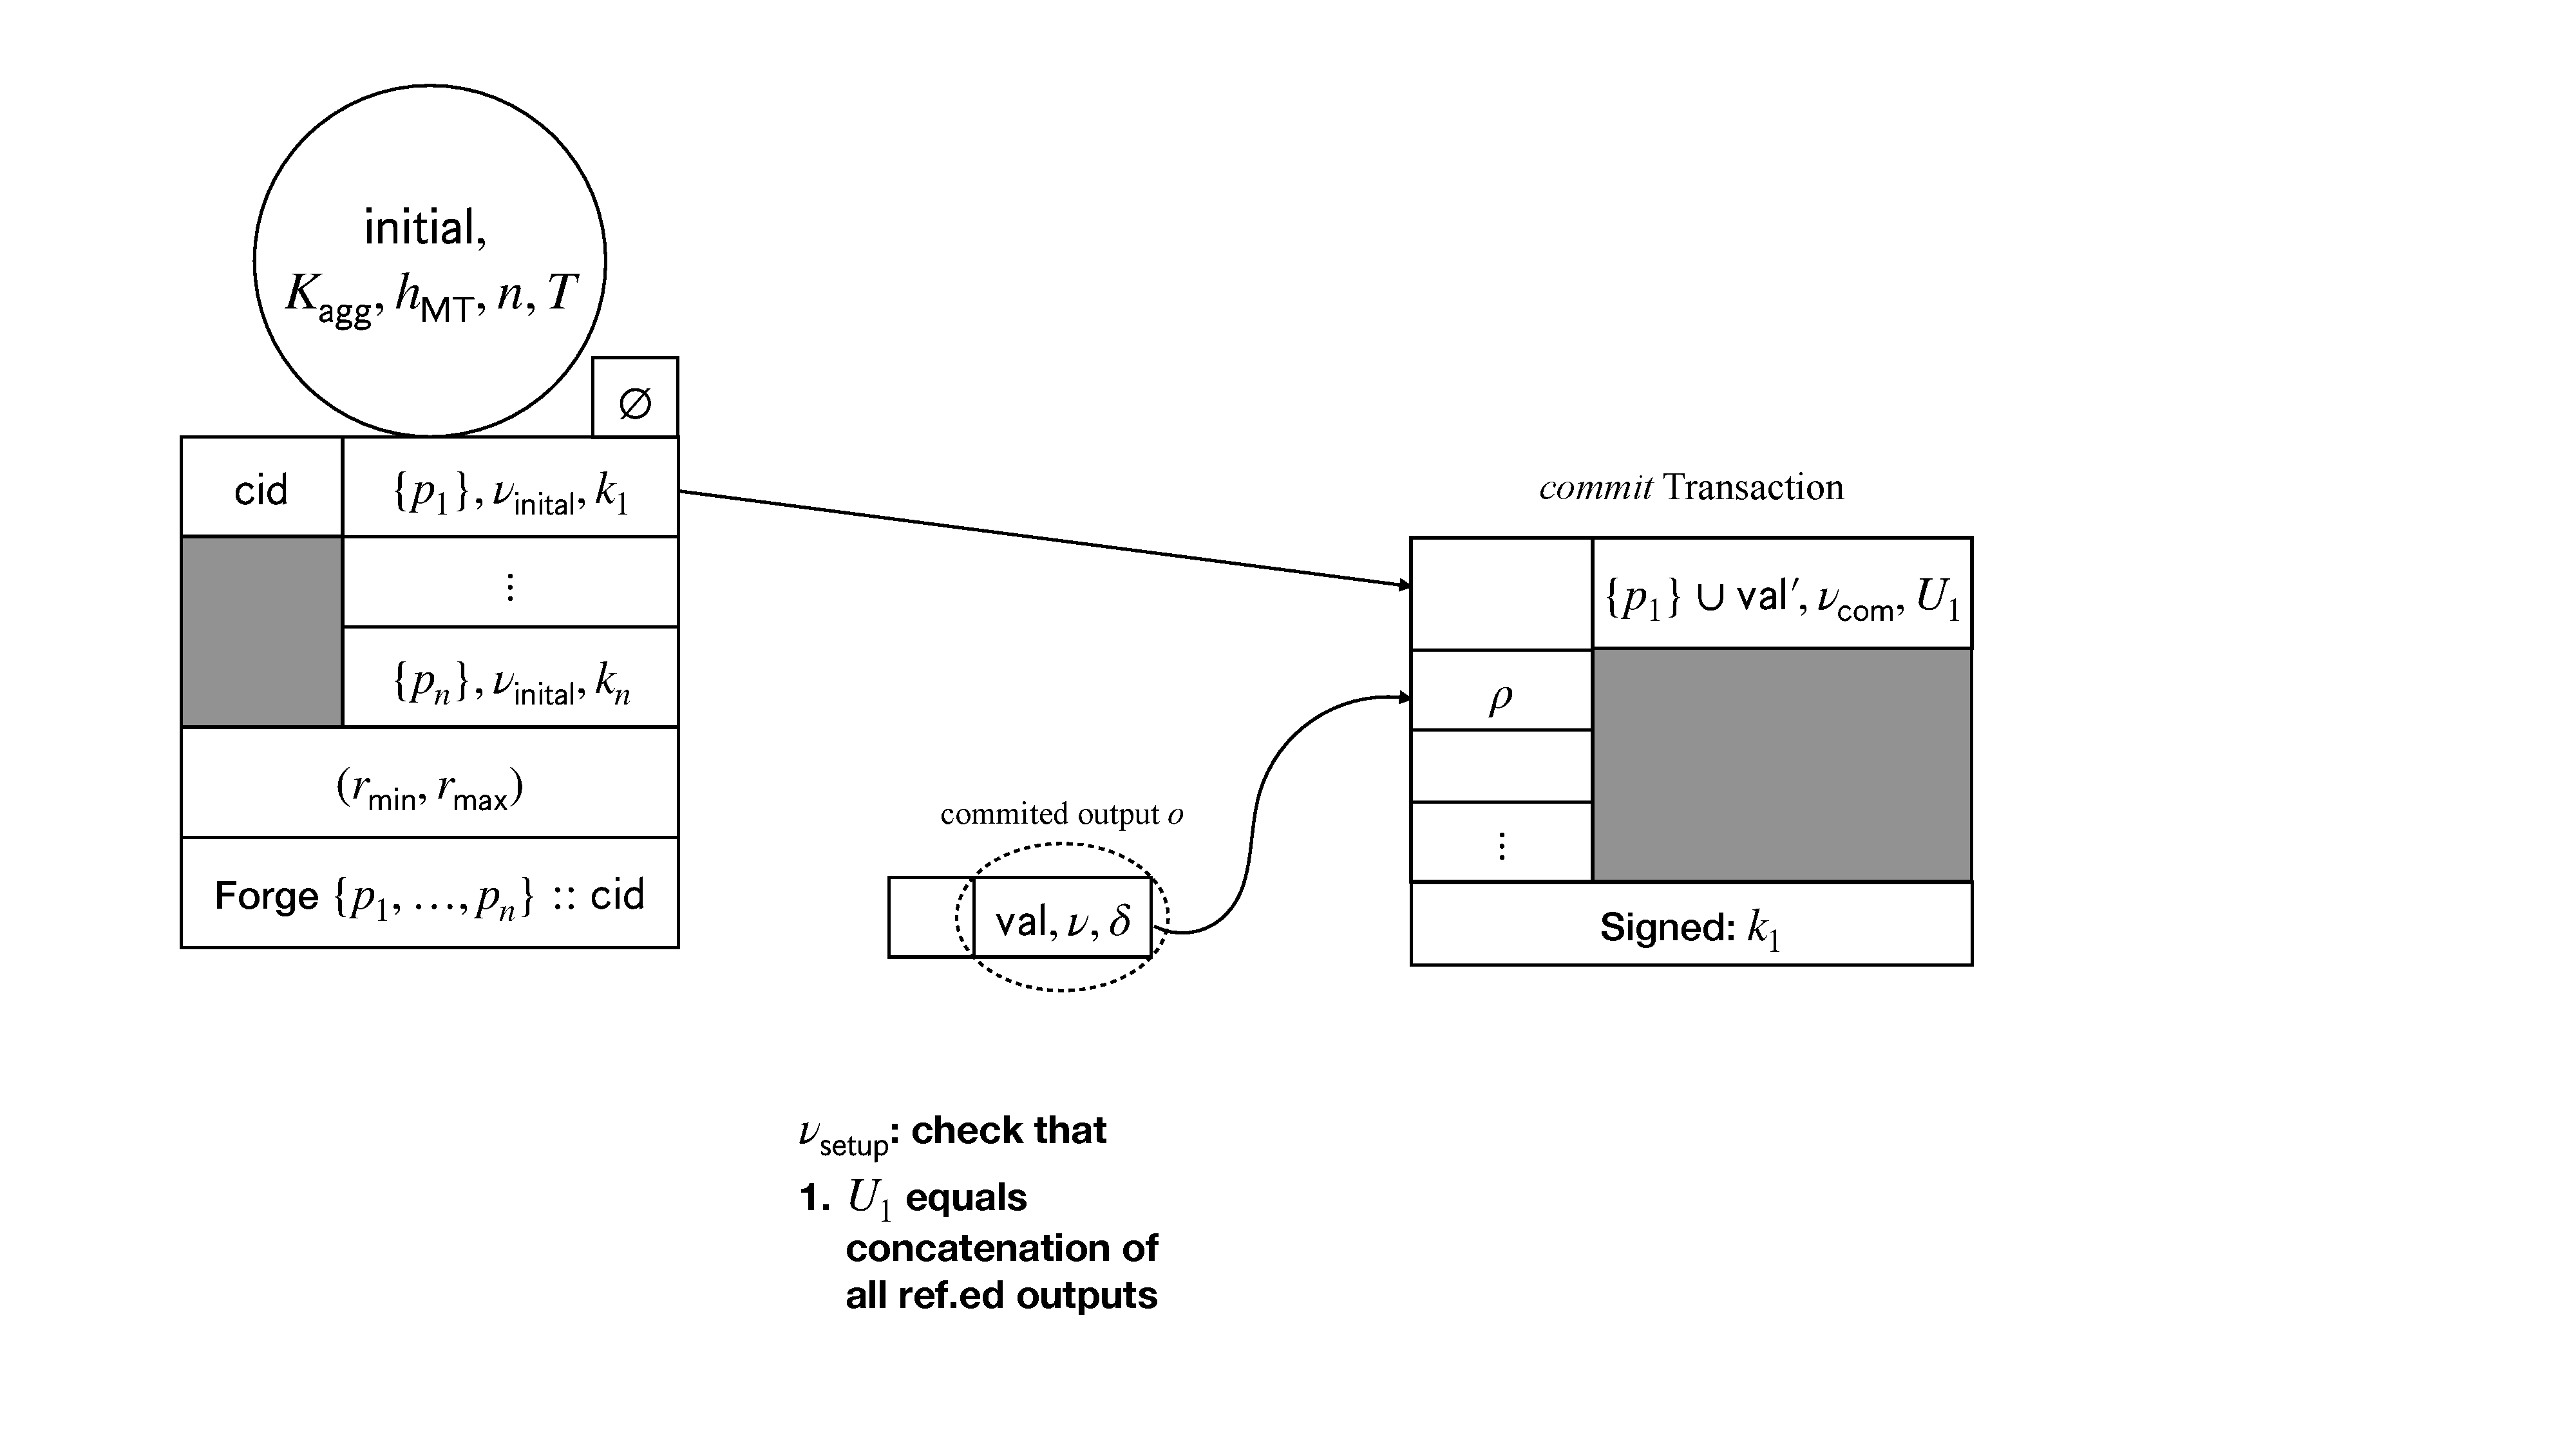
\includegraphics[width=\textwidth/2,trim=130 330 430 50,clip]{figures/SM_commit_tx.pdf}

  % TODO: clean draw marked up version
  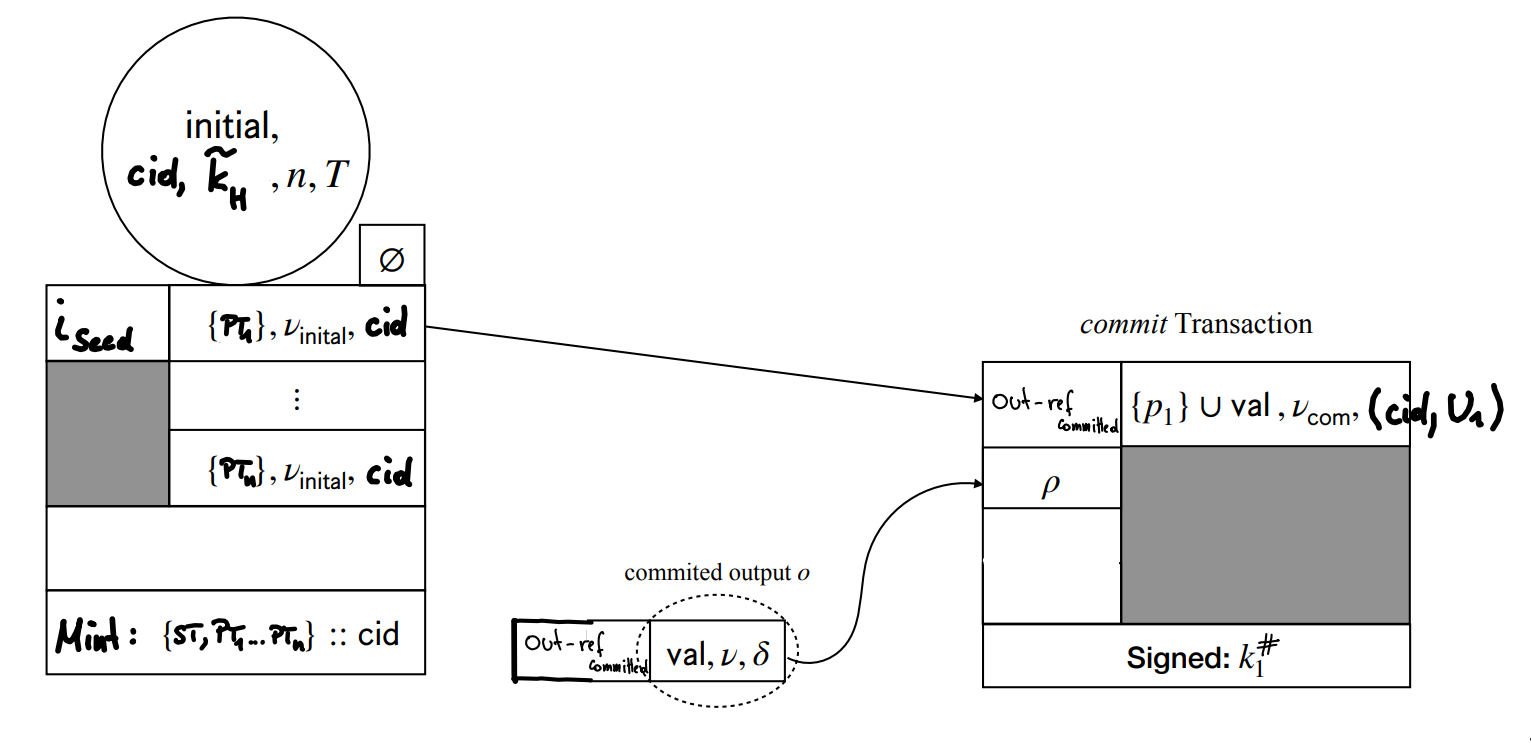
\includegraphics[width=\textwidth*2/3]{figures/SM_commit_tx.png}

  \caption{
    \mtxInit{} transaction (left) with one \mtxCom{} transaction
    (right) attached locking one output (center).}\label{fig:SM_commit_tx}

\end{figure}


%%% Local Variables:
%%% mode: latex
%%% TeX-master: "main"
%%% End:


\subsection{Commit Transaction}\label{sec:commit-tx}

A \mtxCom{} transaction may be submitted by each participant
$\forall i \in \{1 \dots \nop\}$ and is depicted on the right hand side of
Figure~\ref{fig:SM_commit_tx}. It has the following structure:
\begin{itemize}
  \item One input $i_{initial} = (\txOutRef_{initial}, \redeemer_{initial})$
        spending $o_{initial} = (\val_{initial}, \nuInitial, \datum_{initial})$
  \item Zero or one input with reference $\txOutRef_{commit}$ spending output
        $o_{committed} = (\val_{committed}, \cdot , \cdot)$
  \item One output $o_{commit} = (\val_{commit}, \nuCommit, \delta_{commit})$\todo{need to check output address?}
\end{itemize}

\noindent The $\nuInitial$ validator ensures that:
\begin{menumerate}
  \item The initial datum provides the currency id $\cid = \datum_{initial}$
  \item The initial redeemer references the committed output $\redeemer_{initial} = \txOutRef_{committed}$
  \item The committed value is in the output $\val_{com} = \val_{initial} \cup \val_{committed}$
  \item The currencty id and committed output are recorded in the output datum
  $\delta_{commit} = (\cid, U_{i})$ where
  $U_{i} = (\txOutRef_{committed},\bytes(o_{committed}))$
  \item Transaction is signed by a participant $\exists (\cid \rightarrow \keyHash_{i} \rightarrow 1) \in \val_{commit} \Rightarrow \keyHash_{i} \in \txKeys$
  \todo{need to check against head datum ($\hppuv$)?}
  \item No minting or burning  $\txMint = \varnothing$
\end{menumerate}

\noindent The $\nuCommit$ validator ensures the output is collected by either a \mtxCCom{}~\ref{sec:collect-tx} or \mtxAbort{}~\ref{sec:abort-tx} transaction of the on-chain state machine, selected by the appropriate redeemer.

\subsection{CollectCom Transaction}\label{sec:collect-tx}

\begin{figure}[h]

  \centering

  % 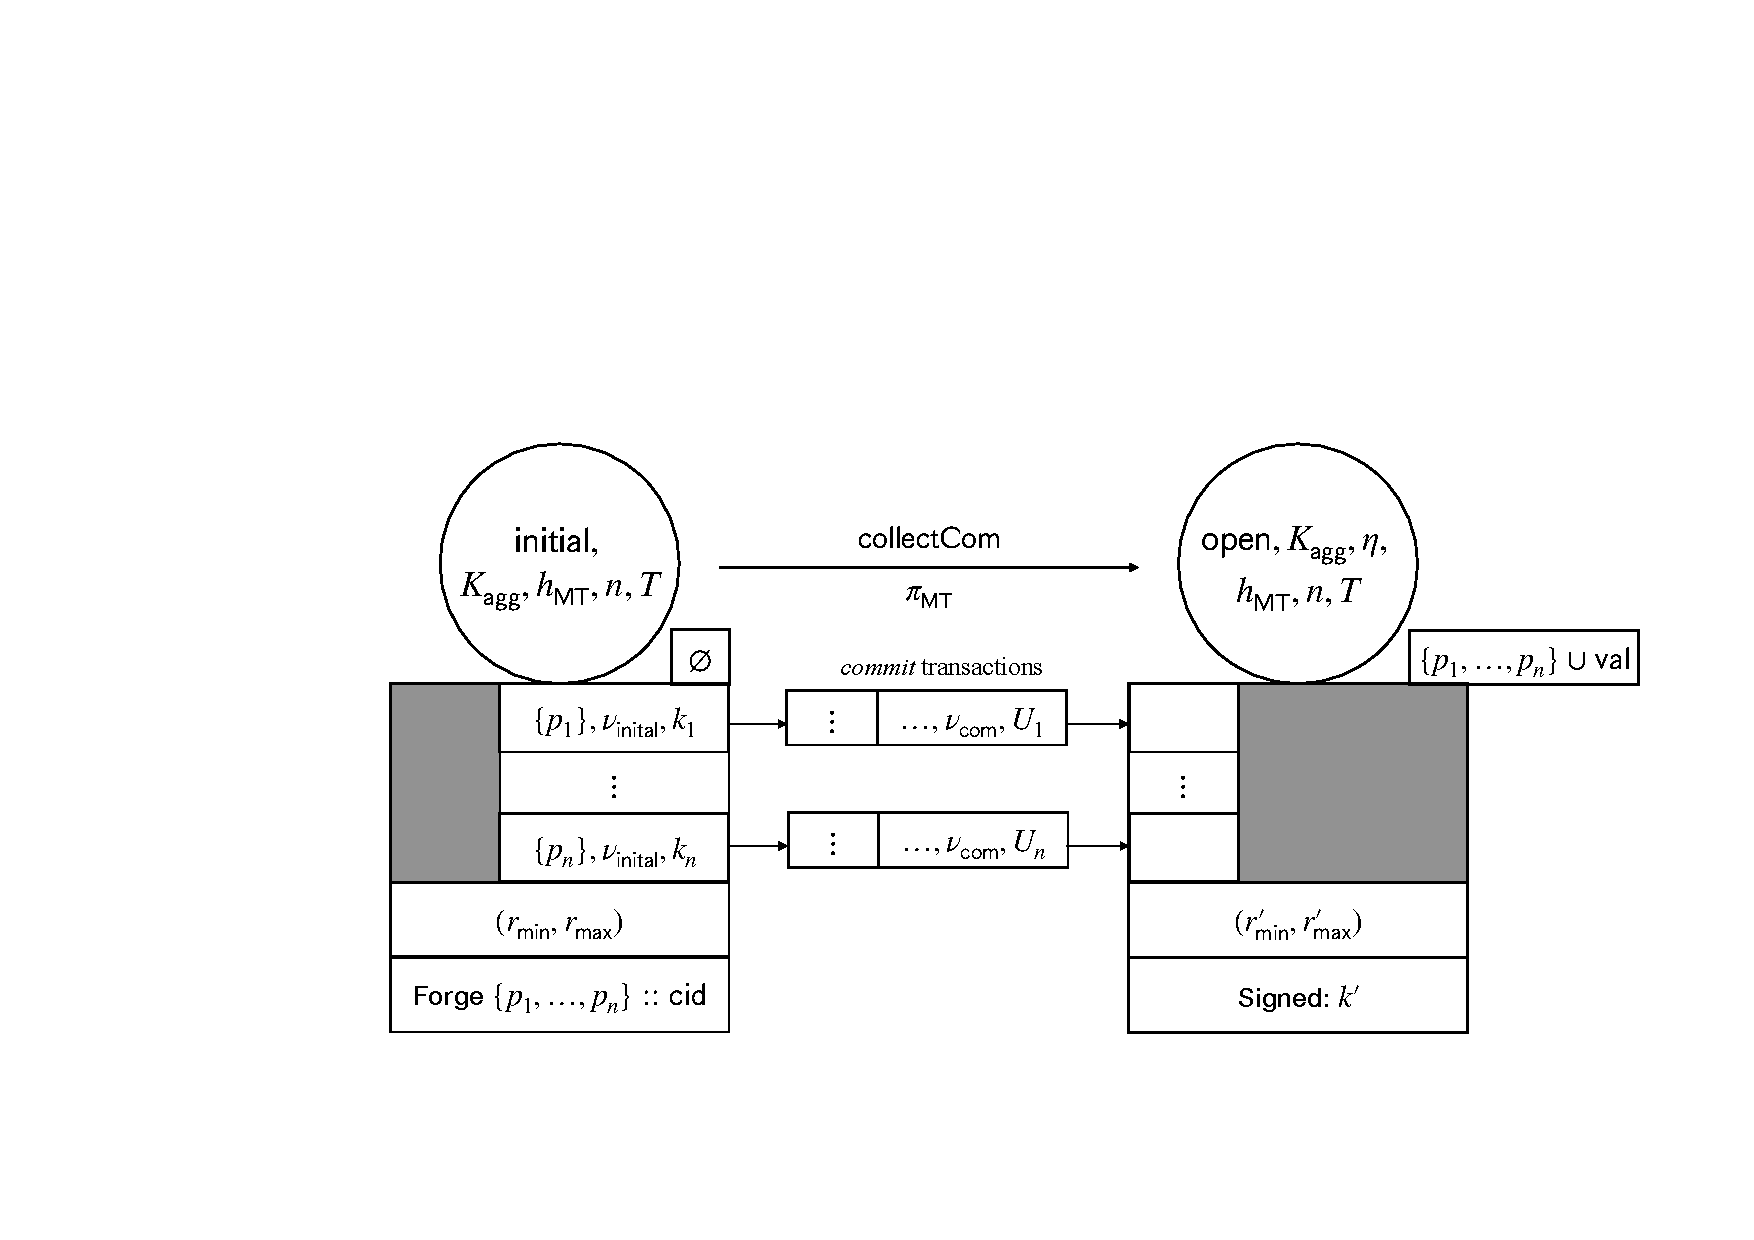
\includegraphics[width=\textwidth/2]{figures/SM_initial_open.pdf}
  %
  % TODO: clean draw marked up version
  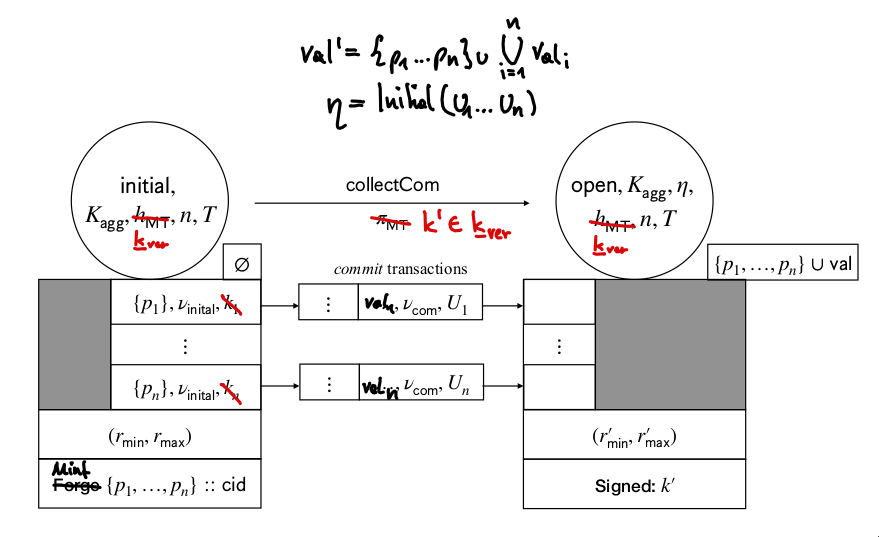
\includegraphics[width=\textwidth/2]{figures/SM_initial_open.png}

  \caption{\mtxInit{} transaction (left) with \mtxCCom{} transaction
    (right) and \mtxCom{} transactions (center).}
  \label{fig:SM_initial_open}

\end{figure}



%%% Local Variables:
%%% mode: latex
%%% TeX-master: "main"
%%% End:


\noindent The \mtxCCom{} transaction collects all the committed UTxOs to the same head. It has
\begin{itemize}
  \item one input spending from $\nuHead$ holding the $\st$, and
  \item $\forall i \in \{1 \dots \nop\}$ inputs spending from \mtxCom{} outputs $(\val_{commit_i}, \nuCommit, (\cid, U_{i}))$ with $\pt_{i} \in \val_{commit_{i}}$.
\end{itemize}
The input spending from and paying to the $\nuHead$ validator, checks the state
of the CEM is advanced:
\[
   (\stInitial,\cid,\hpAK,\hppuv,\nop,\cPer) \xrightarrow{\mathsf{collectCom}} (\stOpen,\cid,\hpAK,\hppuv,\nop,\cPer,\eta)
\]

\noindent Furthermore, $\nuHead$ checks these constraints:
\begin{menumerate}
  \item Collect commits in $\eta$ as the hash, of the concatenation, of
  the serialised representation of committed outputs $U_{i}$, which need to be
  sorted by their associated $\txOutRef$ to be deterministic: \todo{sortByOutRef
    not defined, needed?} \todo{is this clear enough?}
  \[
    \underline{U}_{sorted} = \mathsf{sortByOutRef} ( U_{1}, \dots, U_{\nop} )
  \]
  \[
    \eta = (0, \hash(\bigoplus_{\forall (\cdot, b_{j})~\in~\underline{U}_{sorted}} b_{j}))
  \]
  \item All committed value captured and no additional funds ``enter'' or ``leave''\\
  $\val' = \mathsf{ST} \cup (\bigcup_{i=1}^{n} \val_{commit_i})$
  \item All tokens present in output
  $|\{\cid \rightarrow . \rightarrow 1\} \in \val'| = \nop + 1$\todo{notation? enumerate $\pt_{i}$ using $\hppuv$ instead?}
  \item Transaction is signed by a participant $\exists (\cid \rightarrow \keyHash_{i} \rightarrow 1) \in \val_{commit} \Rightarrow \keyHash_{i} \in \txKeys$\todo{also check $\keyHash_{i} \in \hppuv$?}
  \item Unchanged parameters $\cid$, $\hpAK$, $\hppuv$, $\nop$, and
  $\cPer$ \todo{explicitly state this?}
  \item No minting or burning  $\txMint = \varnothing$
\end{menumerate}

\noindent Each spent $\nuCommit$ validator ensures that:
\begin{menumerate}
  \item The ST token is present in the output value
  $\st = (\cid \rightarrow ``HydraHeadV1'' \rightarrow 1) \in \val'$, where
  $(\cid,\cdot) = \delta_{commit}$ is given by the datum of the commit output
  $o_{commit}$.
\end{menumerate}

\subsection{Abort Transaction}\label{sec:abort-tx}

\begin{figure}

  \centering

  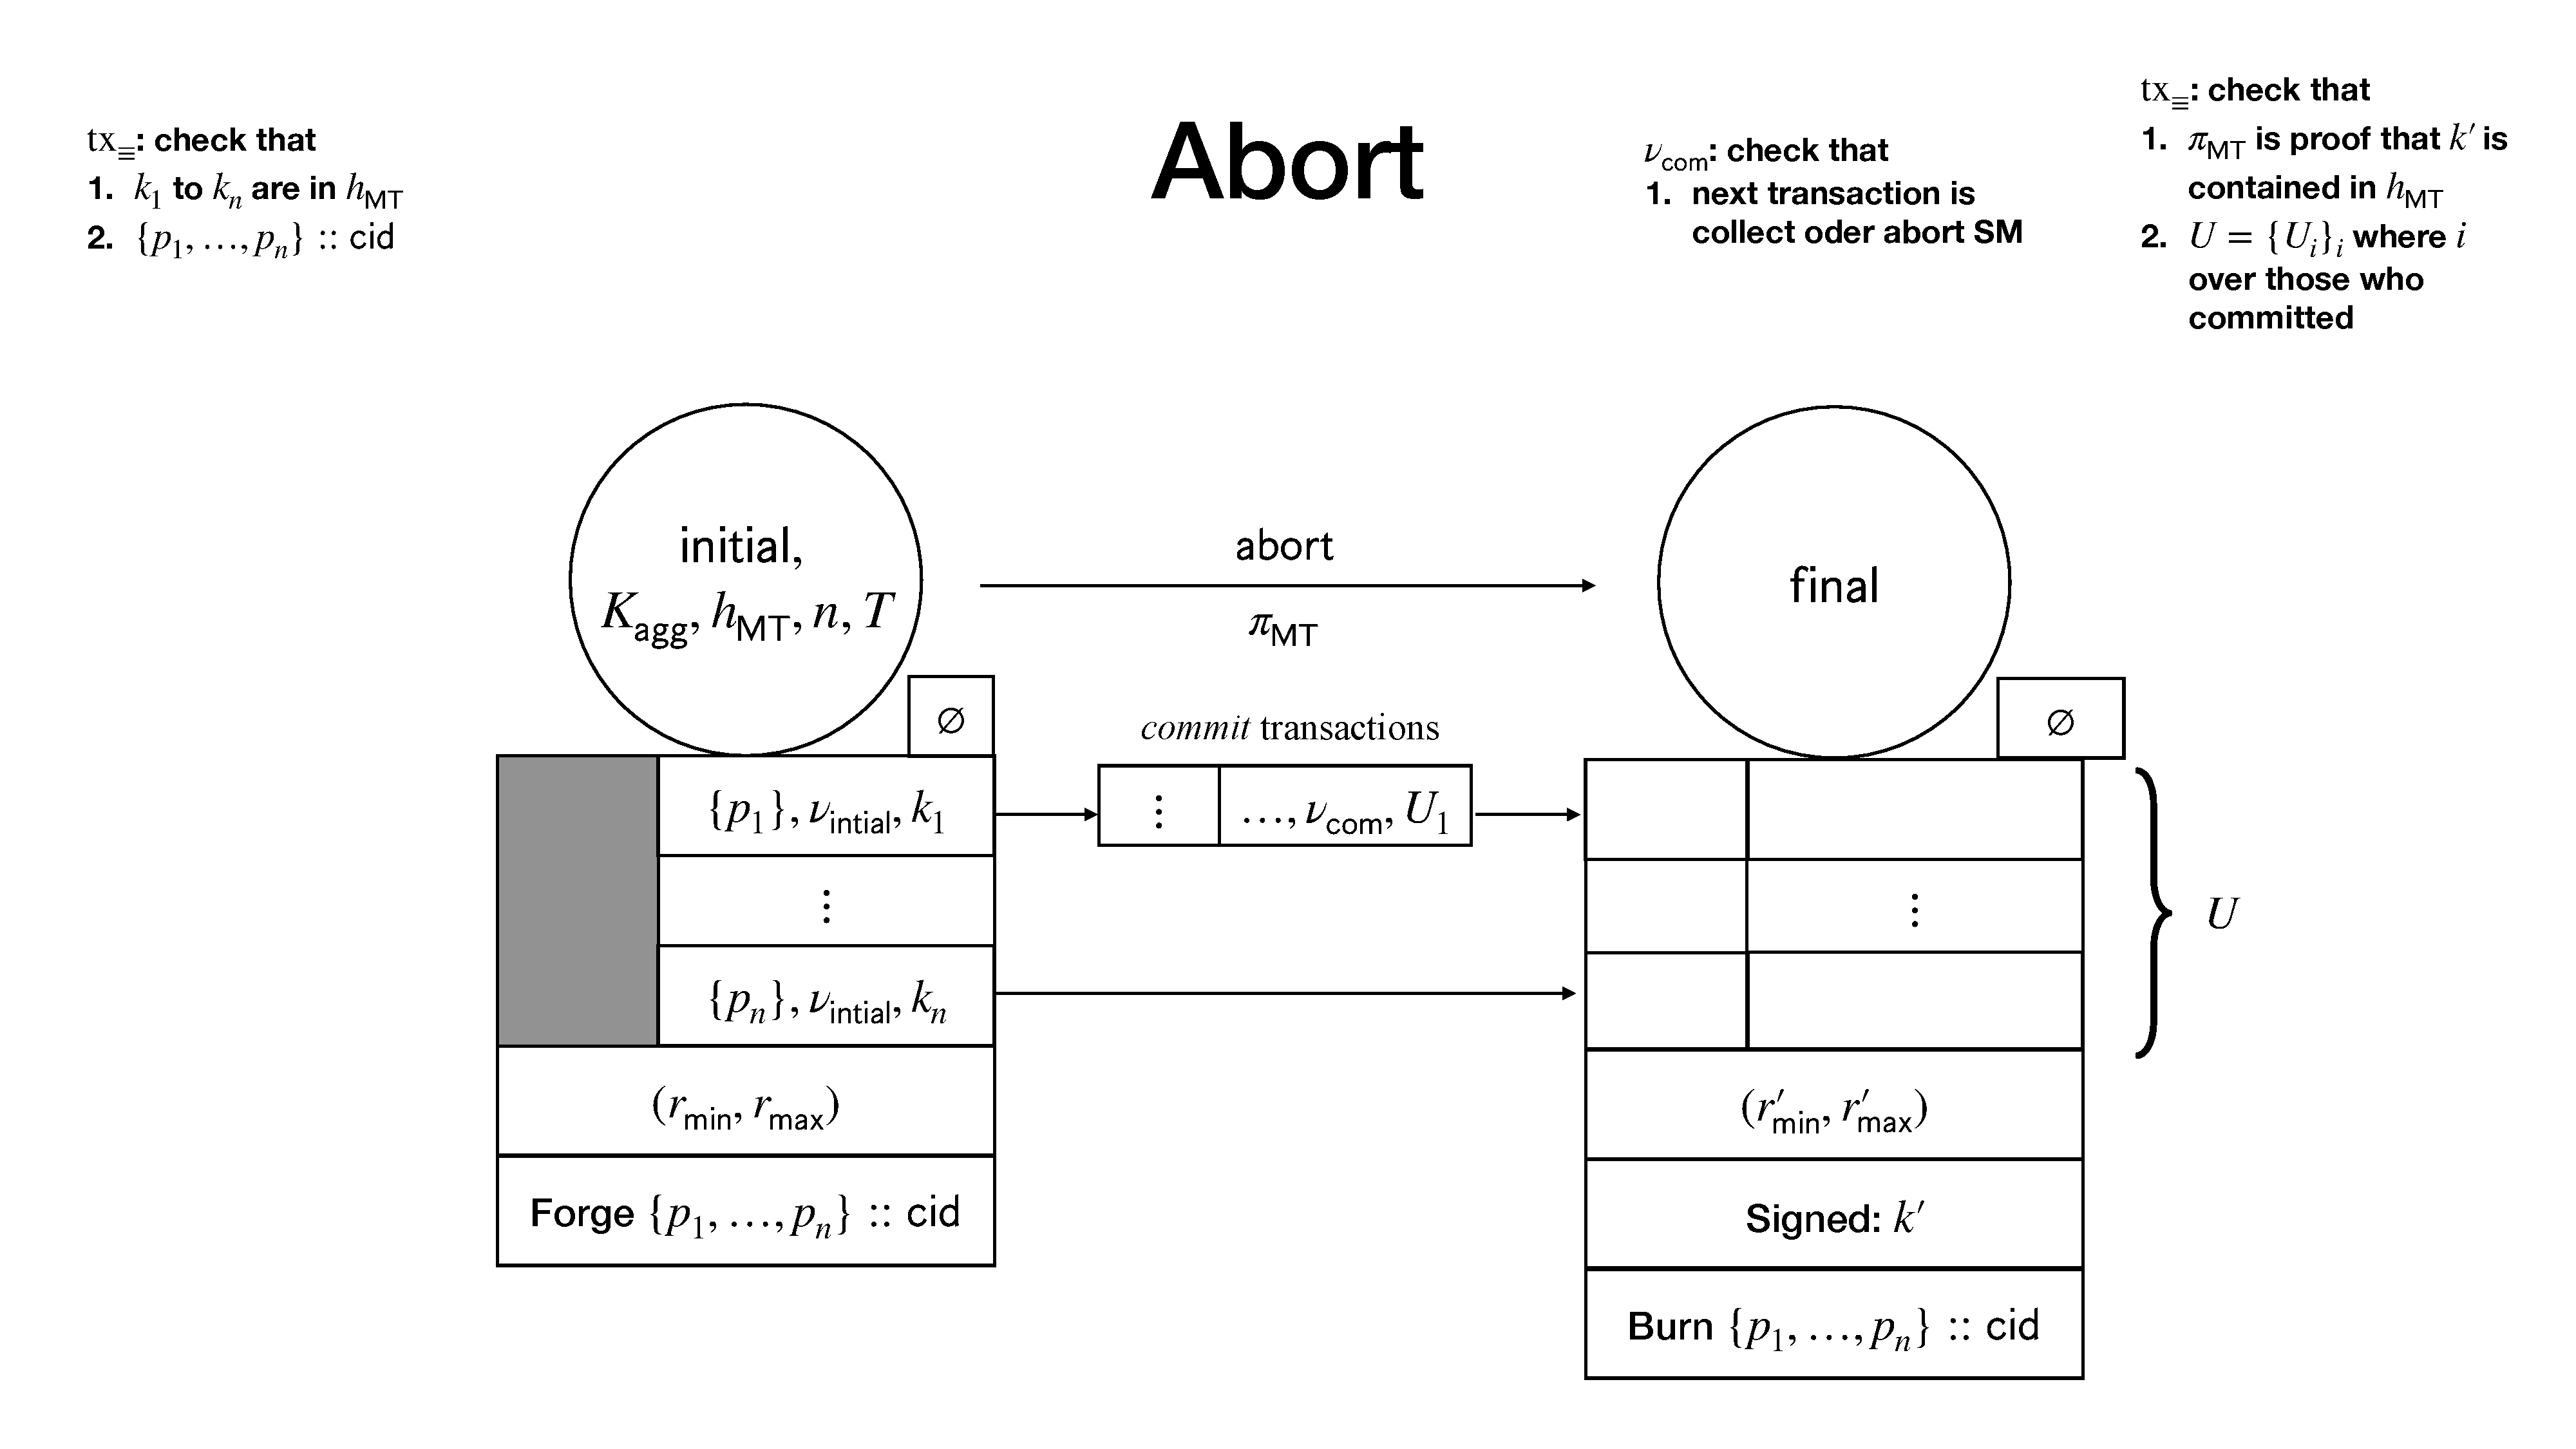
\includegraphics[width=\textwidth/2-2em,trim=350 20 240 300,
  clip]{figures/SM_initial_final.pdf}
    
  \caption{\mtxInit{} transaction (left) with \mtxAbort{} transaction
    (right) and \mtxCom{} transactions (center).}
  \label{fig:SM_initial_final}

\end{figure}



%%% Local Variables:
%%% mode: latex
%%% TeX-master: "main"
%%% End:


The \mtxAbort{} transaction (see Fig.~\ref{fig:SM_initial_final}) allows a party
to abort the creation of a head. It is comprised of
\begin{itemize}
  \item one input spending from $\nuHead$ holding the $\st$, and
  \item $\forall i \in \{1 \dots \nop\}$ inputs either
    \begin{itemize}
      \item spending from an initial output $(\val_{initial_i}, \nuInitial, \cid)$ with $\pt_{i} \in \val_{initial_i}$, or
      \item spending from a commit output $(\val_{commit_i}, \nuCommit, \datum_{commit_i})$ with $\pt_{i} \in \val_{commit_{i}}$,\todo{detail datums below?}
    \end{itemize}
  \item $m$ outputs to redistribute already committed UTxOs.
\end{itemize}
Note that \mtxAbort{} represents a final transition of the CEM and hence there
is no state machine output. The input spending from $\nuHead$ does provide the
number of reimbursed outputs $m$ as redeemer and checks the state of the CEM is
advanced to the final $\stFinal$ as follows:

\[
   (\stInitial,\cid,\hpAK,\hppuv,\nop,\cPer) \xrightarrow[m]{\mathsf{abort}} \stFinal.
\]

\noindent The $\nuHead$ validator ensures that:
\begin{menumerate}
  \item All UTxOs committed into the head are reimbursed exactly as they were
  committed. By comparing hashes of serialised representations of the $m$
  reimbursing outputs\footnote{Only the first $m$ outputs are used for
    reimbursing, while more outputs may be present in the transaction, e.g for
    change} and canonically sorted (by $\txOutRef$) committed UTxOs $U_{i}$ where $(\cdot, U_{i}) = \datum_{commit_{i}}$ from \mtxCom{}~\ref{sec:commit-tx}:
  \todo{list/tuple comprehensions?}
  \[
    \underline{U}_{sorted} = \mathsf{sortByOutRef} ( \forall i \in \{1\dots\nop\} : U_{i} \neq \bot => U_{i})
  \]
  \[
    \hash(\bigoplus_{j}{\underline{U}_{sorted}[j]}^{\downarrow 2}) = \hash(\bigoplus_{j=1}^{m} \bytes(\txOutputs[j]))
  \]

  \item Transaction is signed by a participant $\exists (\cid \rightarrow \keyHash_{i} \rightarrow -1) \in \txMint \Rightarrow \keyHash_{i} \in \txKeys$
 \item All tokens are burnt $|\{\cid \rightarrow \cdot \rightarrow -1\} \in \txMint| = n + 1$\todo{number of tokens burned vs. explicit enumeration what to burn?}
\end{menumerate} 

\noindent Each $\nuInitial$ validator checks:\todo{datums/redeemers here?}
\begin{menumerate}
  \item The ST is getting burned
  $(\cid \rightarrow \texttt{HydraHeadV1} \rightarrow -1) \subseteq \txMint$,
  where $\cid$ is given by the datum of the spent initial output
  $\cid = \delta_{initial}$.
\end{menumerate}

\noindent Each $\nuCommit$ validators checks:
\begin{menumerate}
  \item The ST is getting burned
  $(\cid \rightarrow \texttt{HydraHeadV1} \rightarrow -1) \subseteq \txMint$,
  where $\cid$ is given by the datum of the spent commit output $(\cid,\cdot) = \delta_{commit}$.
\end{menumerate}

\subsection{Close Transaction}\label{sec:close-tx}

\begin{figure}[t!]

  \centering

  %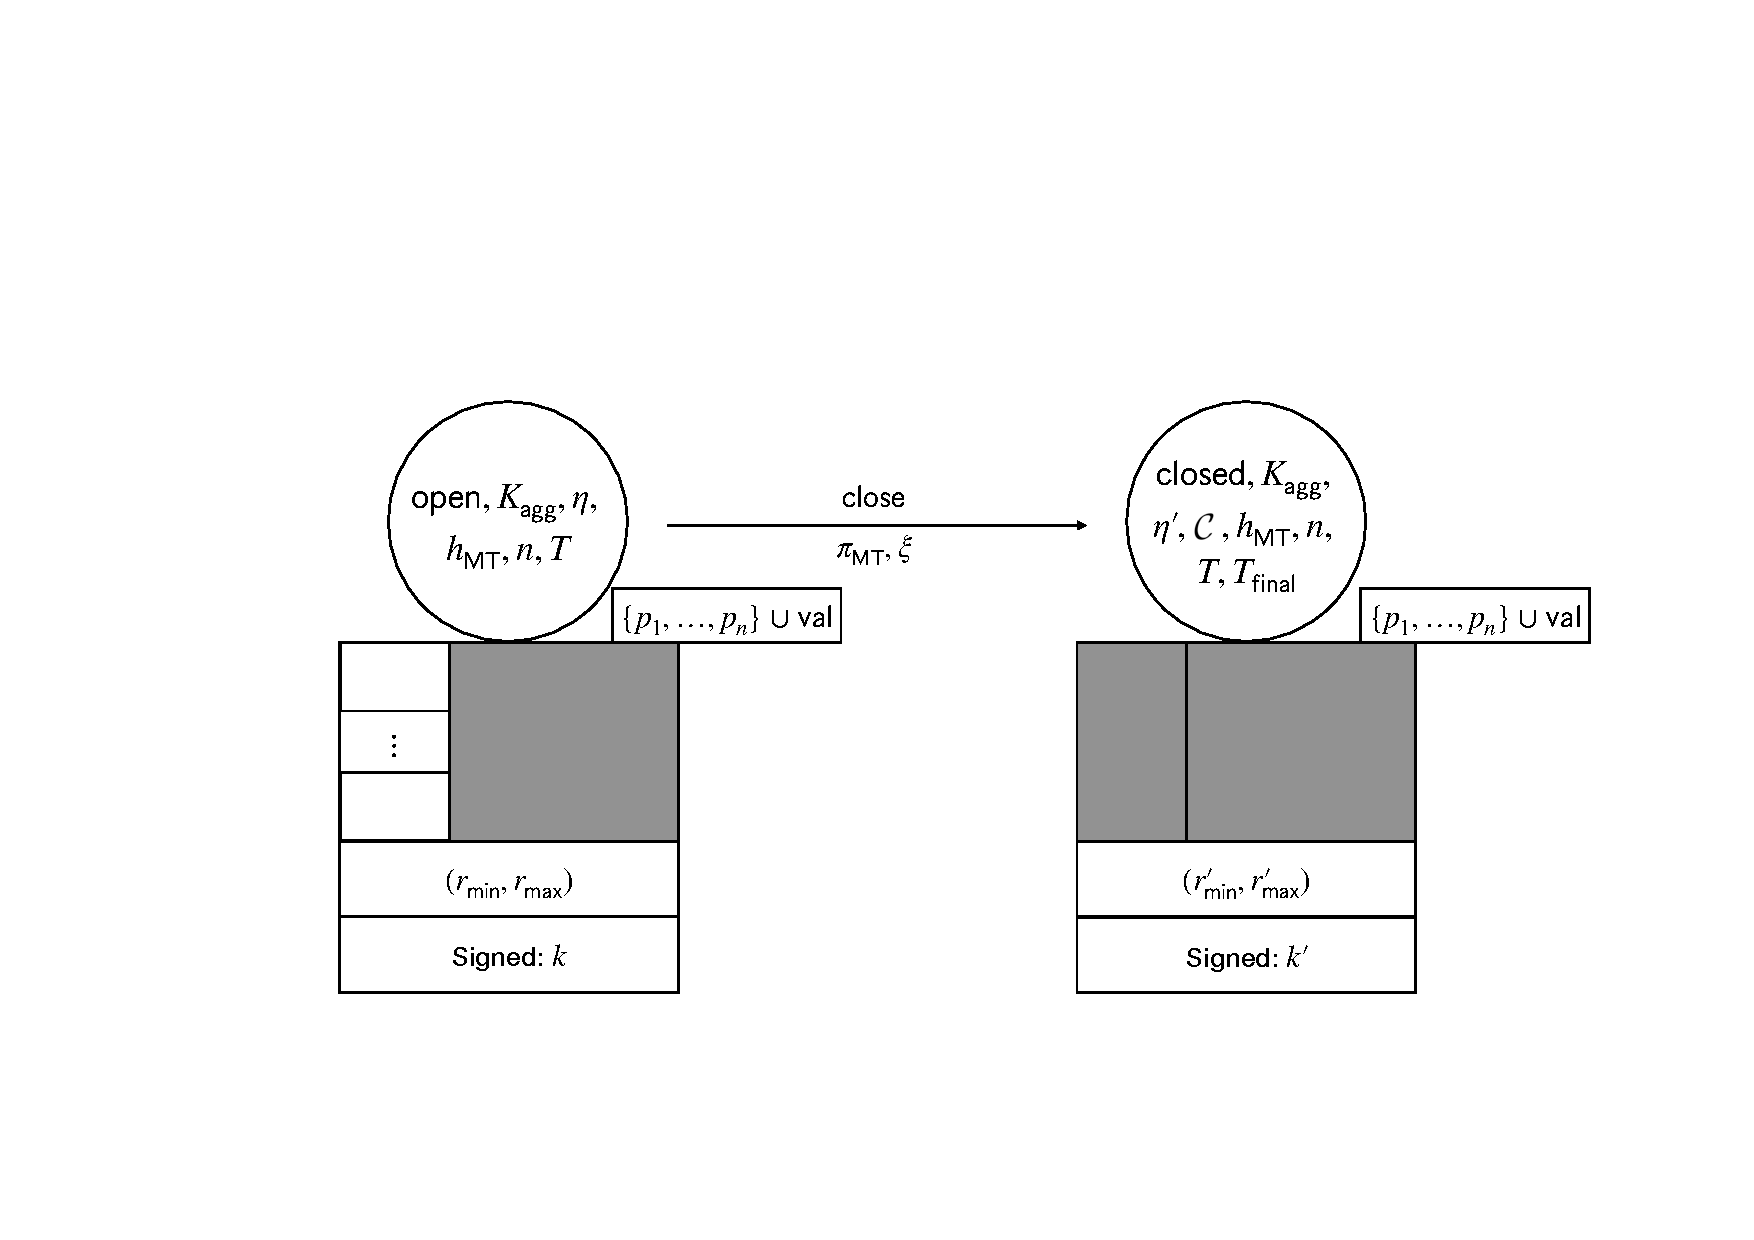
\includegraphics[width=\textwidth/2-2em,trim=350 100 160 300,
  %clip]{figures/SM_open_closed.pdf}

  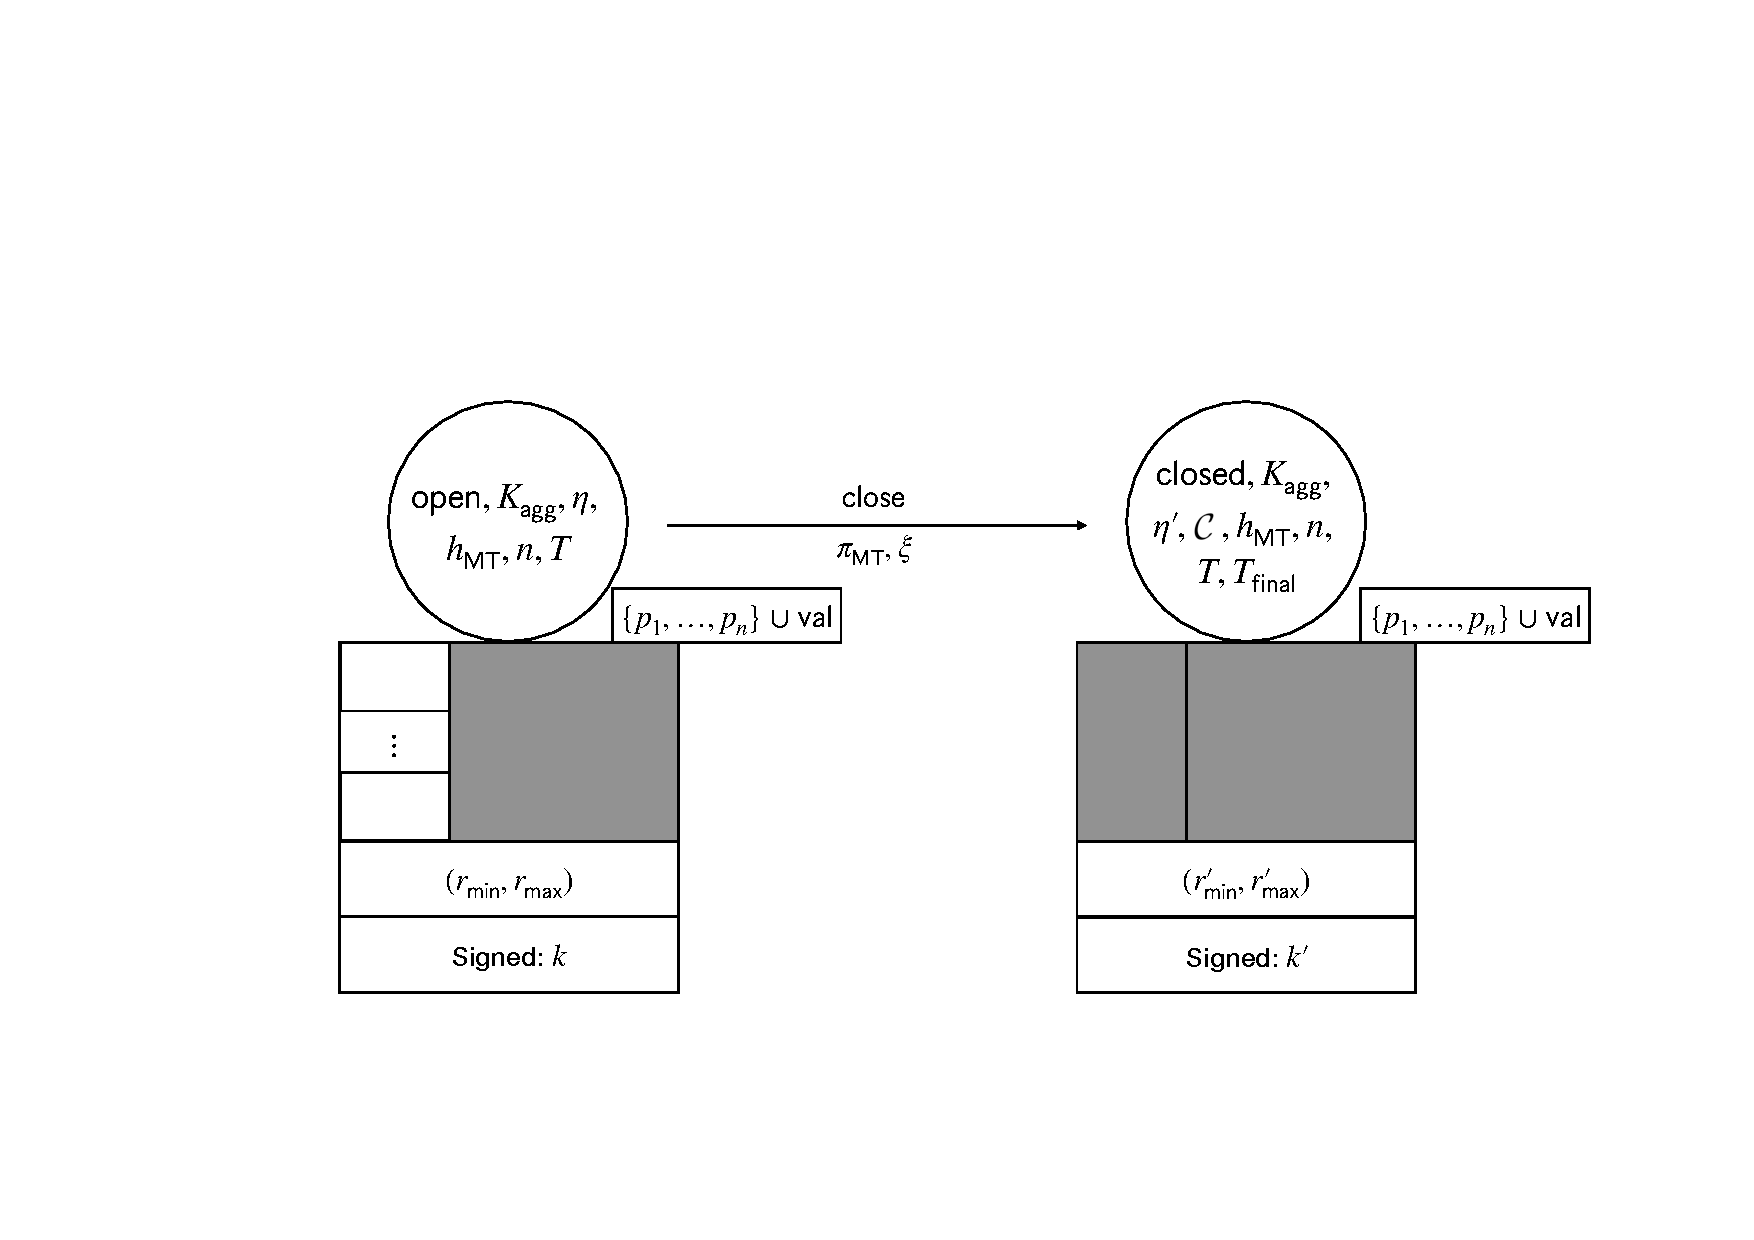
\includegraphics[width=\textwidth/2]{figures/SM_open_closed.pdf}

  \caption{\mtxCCom{} transaction (left) with \mtxClose{}
    transaction (right).}
  \label{fig:SM_open_closed}

\end{figure}



%%% Local Variables:
%%% mode: latex
%%% TeX-master: "main"
%%% End:


In order to close a head, a head member may post the \mtxClose{} transaction
(see Figure~\ref{fig:SM_open_closed}). This transaction has a single input
spending from the $\nuHead$ and paying to the $\nuHead$ validator, which checks
the state of the CEM is advanced:
\[
  (\stOpen,\cid,\hpAK,\hppuv,\nop,\cPer,\eta) \xrightarrow[\xi]{\mathsf{close}} (\stClosed,\cid,\hpAK,\hppuv,\nop,\cPer,\eta_0,\eta',\contesters,\Tfinal)
\]

\noindent The $\nuHead$ validator performs these checks:
\begin{enumerate}
  \item Recorded the initial snapshot state $\eta_0 = \eta$
  \item New snapshot state $(s', U^{\#}') = \eta'$ is the initial $\eta_{0}$
        or correctly signed via $\xi$ \\
        \[
          \left\{\begin{array}{ll}
                  \msVfy(\hpAK,(\cid || \eta_{0} || \eta'),\xi) = \true & \mathrm{if} ~ s' > 0, \\
                  \eta' = \eta_{0} & \mathrm{otherwise}
                 \end{array}\right.
        \]\todo{factor out $s'$?}
  \item Initialize the set of contesters\footnote{This allows the closing party
        to also contest and is required for use cases where pre-signed, valid in
        the future, close transactions are used to delegate head closing}
        $\contesters = \emptyset$
  \item Correct contestation deadline $\Tfinal = \txRmax + T$
  \item Bounded confirmation window\footnote{Ensures head $\Tfinal$ is at most
        $2*T$ in the future} $\txRmax - \txRmin \leq T$
  \item Value in the head is preserved $\val' = \val$
  \item Transaction is signed by a participant $\exists (\cid \rightarrow \keyHash_{i} \rightarrow 1) \in \val' \Rightarrow \keyHash_{i} \in \txKeys$
  \item No minting or burning $\txMint = \varnothing$
\end{enumerate}

\subsection{Contest Transaction}\label{sec:contest-tx}

\begin{figure}

  \centering

  %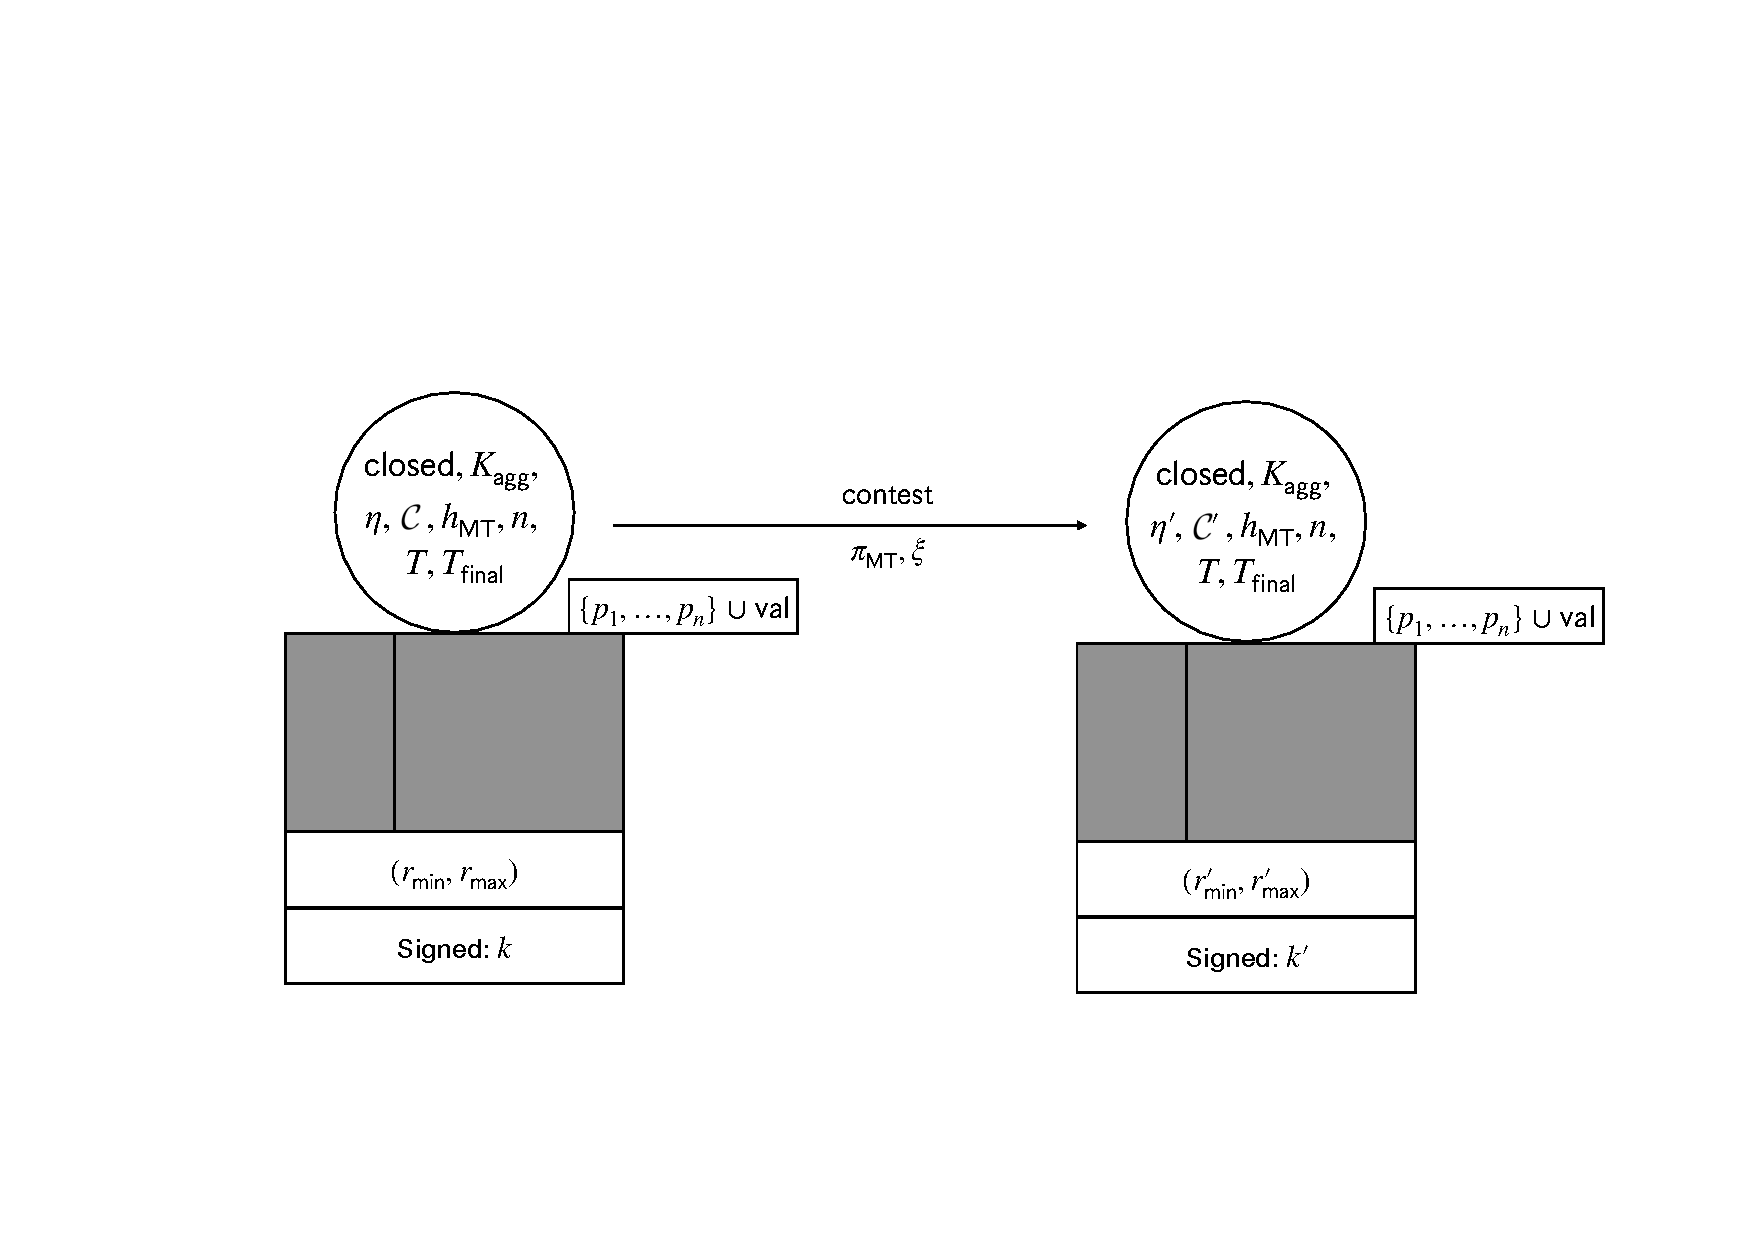
\includegraphics[width=\textwidth/2-2em,trim=280 120 160 260,
  %clip]{figures/SM_closed_closed.pdf}

  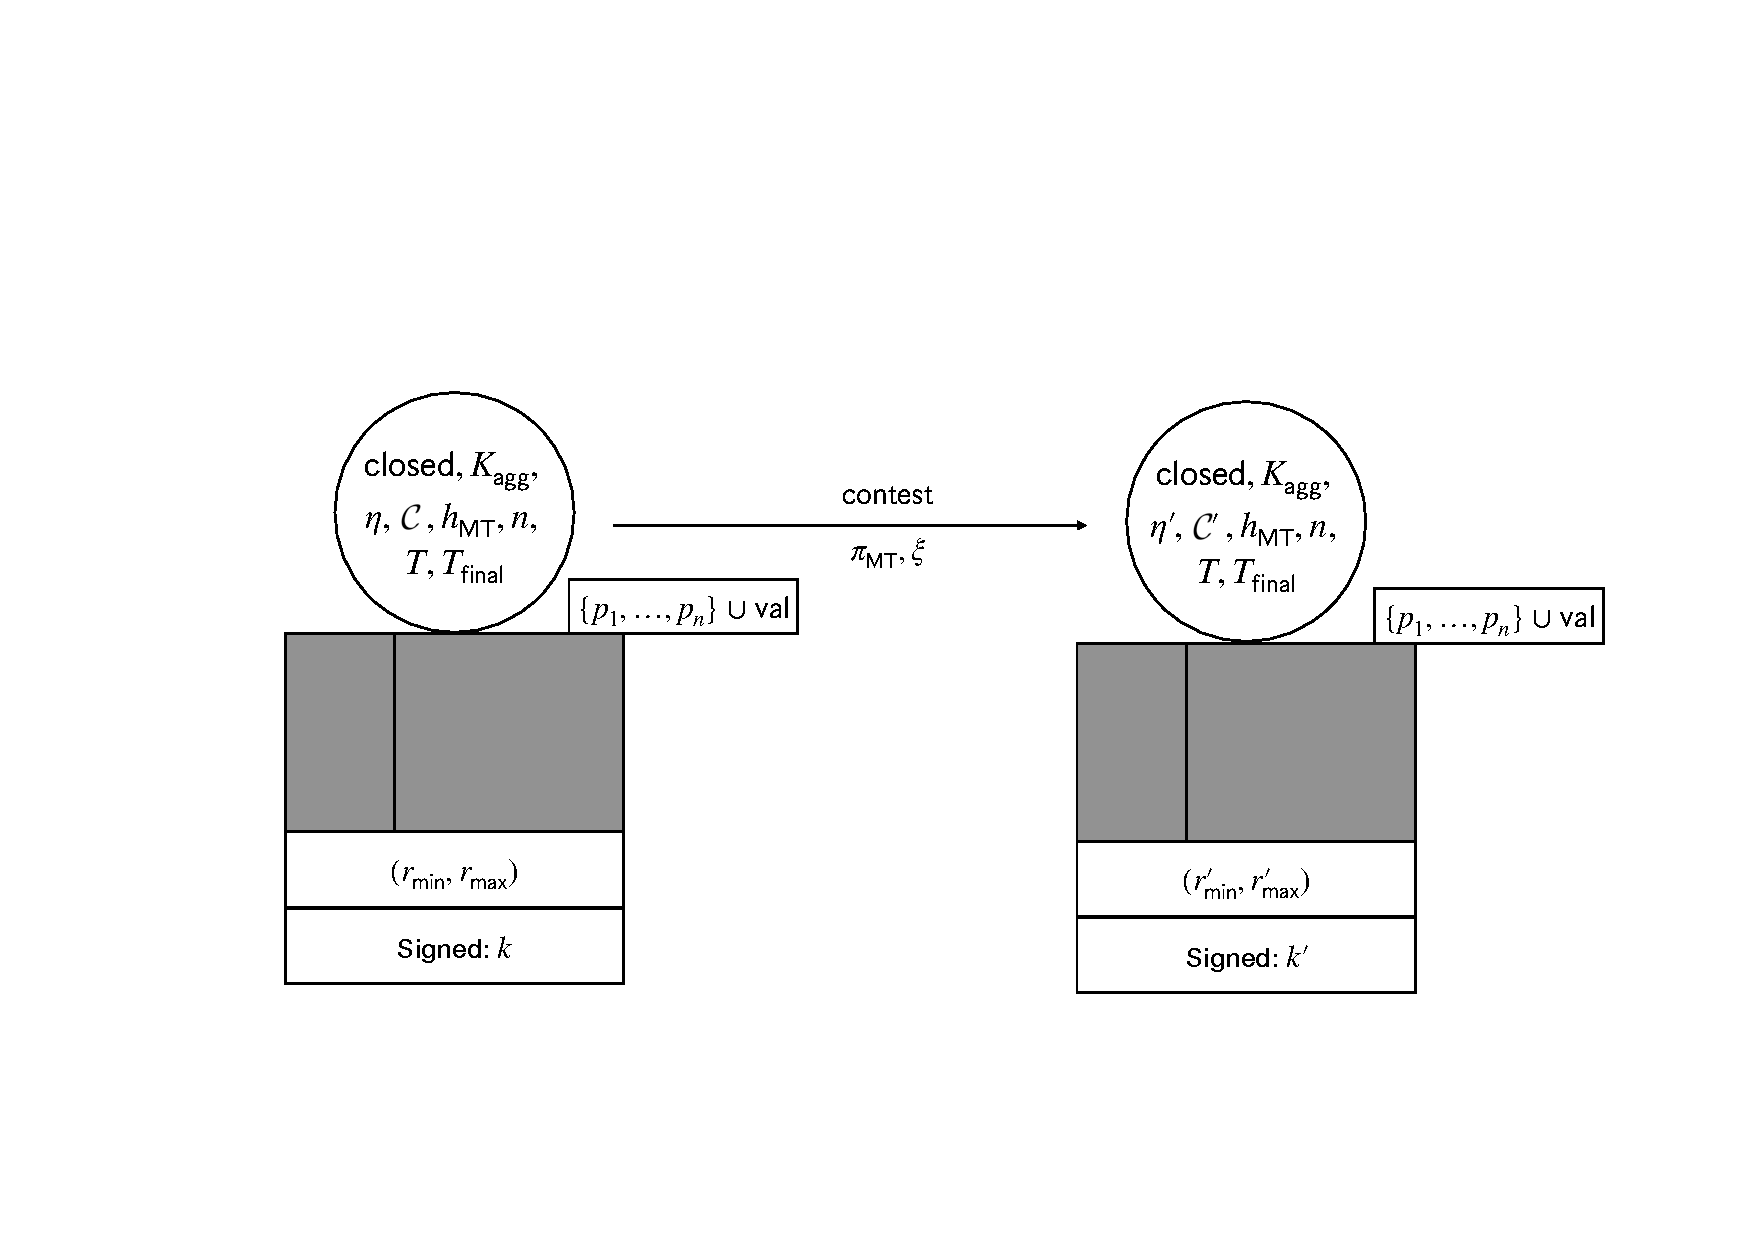
\includegraphics[width=\textwidth/2]{figures/SM_closed_closed.pdf}

  \caption{\mtxClose{}/\mtxContest{} transaction (left);
    \mtxContest{} transaction (right)}
  \label{fig:SM_closed_closed}

\end{figure}



%%% Local Variables:
%%% mode: latex
%%% TeX-master: "main"
%%% End:


The \mtxContest{} transaction (see Figure~\ref{fig:SM_closed_closed}) is posted
by a party to prove the currently $\stClosed$ state is not the latest one. This
transaction has a single input spending from the $\nuHead$ and paying to the
$\nuHead$ validator, which checks the state of the CEM is advanced:
\[
  (\stClosed,\cid,\hpAK,\hppuv,\nop,\cPer,\eta_0,\eta,\contesters,\Tfinal) \xrightarrow[\xi]{\mathsf{contest}} (\stClosed,\cid,\hpAK,\hppuv,\nop,\cPer,\eta_0,\eta',\contesters',\Tfinal')
\]

\noindent The $\nuHead$ validator performs these checks:
\begin{menumerate}
  \item Contest snapshot is newer $s' > s$, where $(s, \cdot) = \eta$ is the current and $(s', \cdot) = \eta'$ is the contest snapshot number
  \item $\xi$ is a valid multi-signature of the new snapshost state
  $\msVfy(\hpAK,(\cid || \eta_{0} || \eta'),\xi) = \true$
  \item The single signer $\{\keyHash\} = \txKeys$ has not already contested $\keyHash \not\in \contesters$ and is added to the set of contesters $\contesters' = \contesters \cup \keyHash$
  \item Transaction is posted before deadline $\txRmax \leq \Tfinal$
  \item Contestation deadline is updated correctly
     \[
       \Tfinal' = \left\{\begin{array}{ll}
                           \Tfinal     & \mathrm{if} ~ |\contesters'| = n, \\
                           \Tfinal + T & \mathrm{otherwise}
                         \end{array}\right.
    \]
  \item Transaction is signed by a participant $\exists (\cid \rightarrow \keyHash_{i} \rightarrow 1) \in \val' \Rightarrow \keyHash_{i} \in \txKeys$
  \item Value in the head is preserved $\val' = \val$
  \item No minting or burning $\txMint = \varnothing$
\end{menumerate}

\subsection{Fan-Out Transaction}
\todo{Mention this is a final state / has no state machine output}

\begin{figure}

  \centering

  % 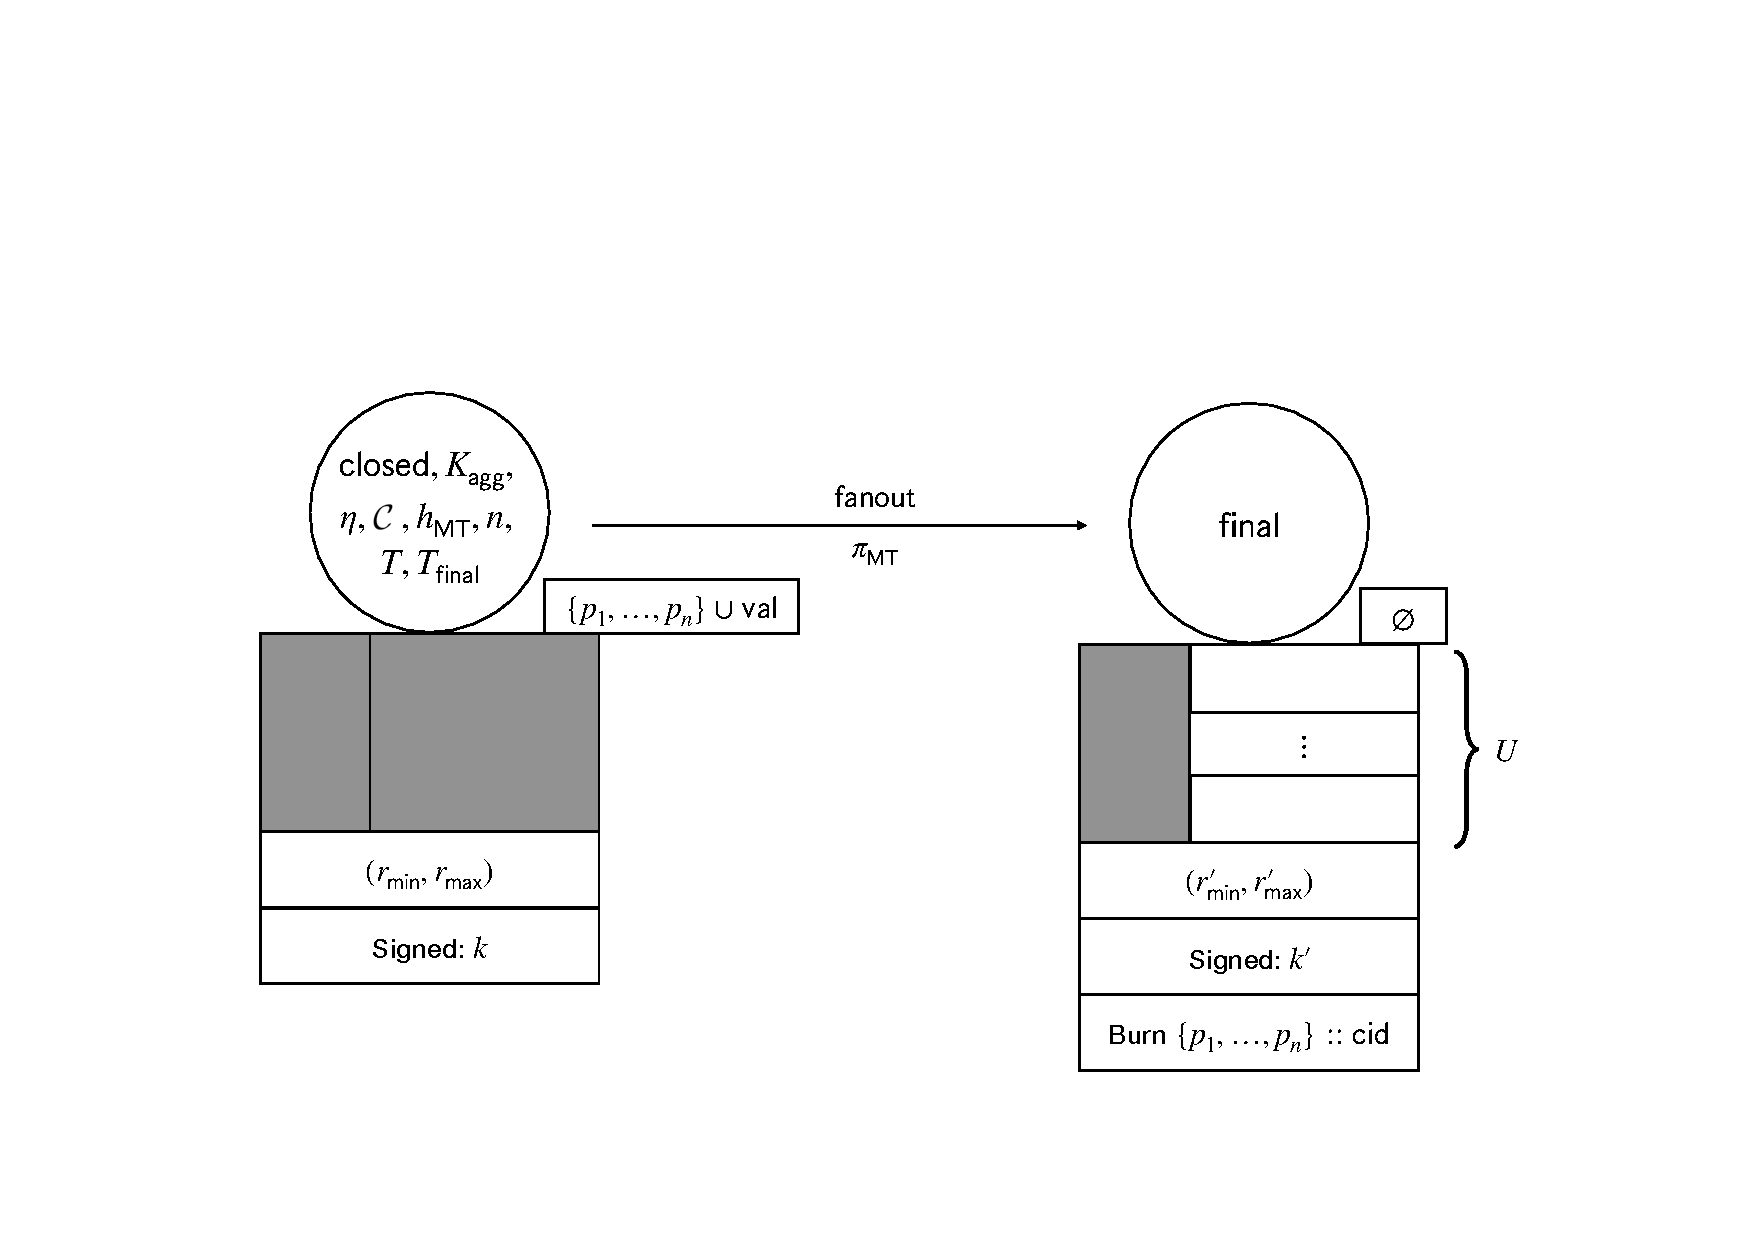
\includegraphics[width=\textwidth/2]{figures/SM_closed_final.pdf}

  % TODO: clean draw marked up version
  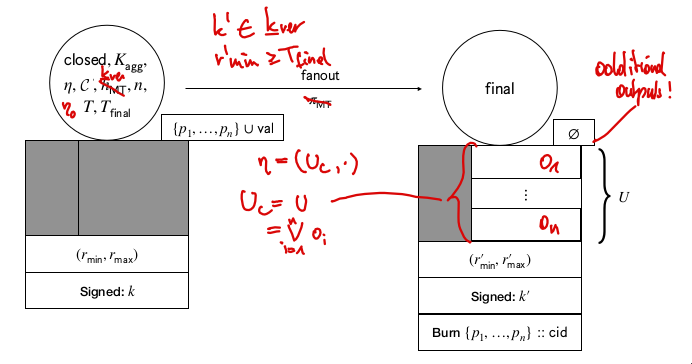
\includegraphics[width=\textwidth/2]{figures/SM_closed_final.png}

  \caption{\mtxClose{}/\mtxContest{} transaction (left);
    \mtxFanout{} transaction (right)}\label{fig:SM_closed_final}

\end{figure}

%%% Local Variables:
%%% mode: latex
%%% TeX-master: "main"
%%% End:


Once the contestation phase is over, a head
may be finalized by posting a \mtxFanout{} transaction, taking the SM
from $\stClosed$ to $\stFinal$.  

$$
   (\stClosed,\hpAK,\eta,\eta_0,\contesters,\hppuv,\nop,\cPer,\Tfinal) \xrightarrow{\mathsf{fanout}} \stFinal,
$$
with $\eta = (s, H)$ and $\eta_0 = (0, H_0).$
The $\nuHead$ validator performs the following checks:
\begin{enumerate}
  \item Correct outputs are created: 
  $$
  \hash(\bigoplus_{i=1}^n \bytes(O[i])) = 
    \left\{
    \begin{array}{ll}
        H_0, & s = 0 \\
        H, &\mathit{otherwise}
    \end{array}
    \right.,
  $$
  % TODO: use this in fanout
  % \[
  %   \hash(\bigoplus_{j=1}^{m} \bytes(\txOutputs[j])) = \eta
  % \]

  \item All tokens are burnt: 
     $\mathsf{ST} \cup \{(\cid \rightarrow \mathsf{PT}_i \rightarrow -1) \mid i \in \{1\dots\nop\}\} \subseteq \mathsf{Mint},$
  \item Transaction is posted after contestation deadline $\txRmin > \Tfinal.$
\end{enumerate}

%%% Local Variables:
%%% mode: latex
%%% TeX-master: "main"
%%% End:
